\section{Online Adversarial Attacks}
\label{online_adversarial_attacks}
\looseness=-1
Motivated by our more realistic threat model, we now consider a novel adversarial attack setting where the data is no longer static but arrives in an online fashion.

\subsection{Adversarial Attacks as Secretary Problems}
\looseness=-1
\label{adv_sec_problem}
The defining feature of the online threat model---in addition to streaming data and the fact that we may not have access to the target model $f_t$---is the online attack budget constraint.
Choosing when to attack under a fixed budget in the online setting can be related to a secretary problem. We formalize this online adversarial attack problem in the boxed online threat model below.

In the online threat model we are given a data stream $\mathcal{D}=\{(x_1,y_1),\ldots,(x_n,y_n)\}$ of $n$ samples ordered by their time of arrival. In order to craft an attack against the target model $f_t$, the adversary selects, using its online algorithm $\mathcal{A}$, a subset $S_{\mathcal{A}} \subset \mathcal{D}$ of items to maximize: %\footnote{$S_{\mathcal{A}}$ contains either indexes or elements of the datastream.}
\begin{equation}\label{eq:asp}
   \setvaluemath(S_\mathcal{A}) \! := \!\!\! \sum_{ (x,y) \in S_\mathcal{A}} \ell(f_{t}(\textsc{Att}(x)),y) \ \text{ s.t. } 
   |S_A| \leq k,\hspace{-1mm} 
\end{equation}
\cut{
\begin{equation}\label{eq:asp}
   \setvaluemath(S_\mathcal{A}) \! := \!\!\! \sum_{ i \in S_\mathcal{A}}v_i \text{ s.t. }  v_i = \ell(f_{t}(x_i'),y_i) \text{ and }
   |S_A| \leq k,\hspace{-1mm} 
\end{equation}
}
where $\textsc{Att}(x)$ denotes an attack on $x$ crafted by a \emph{fixed} attack method $\textsc{Att}$ that might or might not depend on $f_t$. From now on we define $x_i'=\textsc{Att}(x_i)$. 
Intuitively, the adversary chooses $k$ instances that are the ``easiest" to attack, i.e. samples with the highest value. Note that selecting an instance to attack does not guarantee a successful attack.
Indeed, a successful attack vector may not exist if the perturbation budget $\gamma$ is too small. \cut{even though the value is maximized.} However, stating the adversarial goal as maximizing the value of $S_{\mathcal{A}}$ leads to the measurable objective of calculating the ratio of successful attacks in $S_{\mathcal{A}}$ versus $S^*$.

If the adversary knows the true value of a datapoint then the online attack problem reduces to the original $k$-secretary. On the other hand, the adversary might not have access to $f_t$ and instead, the adversary's value function may be an estimate of the true value---e.g.\ the loss of a surrogate classifier, and the adversary must make selection decisions in the face of uncertainty.\cut{ yielding a stochastic generalization of the $k$-secretary problem.} The theory developed in this paper will tackle both the case where values $v_i:=\ell(f_t(x_i'),y_i)$ for $i \in \{1,\ldots,n\} :=[n]$ are known (\S\ref{virtual_plus}), as well as the richer stochastic setting with only estimates of $v_i\,,\, i \in [n]$ (\S\ref{stochastic_k_secretary}).


\xhdr{Practicality of the Online Threat Model} It is tempting to consider whether in practice the adversary should forego the online attack budget and instead attack every instance. However, such a strategy poses several critical problems when operating in real-world online attack scenarios. Chiefly, attacking any instance in $\mathcal{D}$ incurs a non-trivial risk that the adversary is detected by a defense mechanism. Indeed, when faced with stateful defense strategies (e.g. \cite{chen2020stateful}) every additional attacked instance further increases the risk of being detected and rendering future attacks impotent. Moreover, attacking every instance may be infeasible computationally for large $n$ or impractical based on other real-world constraints. Generally speaking, as conventional adversarial attacks operate by restricting the perturbation to a fraction of the maximum possible change (e.g., $\ell_{\infty}$-attacks) online attacks analogously restrict the time window to a fraction of possible instances to attack. Similarly, knowledge of $n$ is also a factor that the adversary can easily control in practice. For instance, in the autonomous control system example, the adversary can choose to be active for a short interval---e.g., when the autonomous car is a certain geospatial location---and thus set the value for $n$.

\begin{ftheo}
The online threat model relies on the following key definitions:
\begin{itemize}[leftmargin=*, itemsep=1pt, topsep=1pt, parsep=1pt]
\item 
\textbf{The target model $f_t$}. The adversarial goal is to attack some target model $f_t : \mathcal{X} \rightarrow \mathcal{Y}$, through adversarial examples that respect a chosen distance function, $d$, with tolerance $\gamma$. %--i.e. $d(x,x') \leq \gamma$ 

\item
\textbf{The data stream $\mathcal{D}$}. The data stream $\mathcal{D}$ contains the $n$ examples $(x_i,y_i)$ ordered by their time of arrival. At any timestep $i$, the adversary receives the corresponding item in $\mathcal{D}$ and must decide whether to execute an attack or forever forego the chance to attack this item.

\item
\textbf{Online attack budget $k$}. The adversary is limited to a maximum of $k$ attempts to craft attacks within the online setting thus imposing that each attack is on a unique item in $\mathcal{D}$.

\item
\textbf{A value function $\mathcal{V}$}. Each item in the dataset is assigned a value on arrival by the value function $\mathcal{V}: \mathcal{X} \times \mathcal{Y} \rightarrow \mathbb{R}_+$ which represents the utility of selecting the item to craft an attack. This can be the likelihood of a successful attack under $f_t$ (true value) or a stochastic estimate of the incurred loss given by a surrogate model $f_s \approx f_t$.
\end{itemize}

The online threat model corresponds to the setting where the adversary seeks to craft adversarial attacks (i) against a target model $f_t \in \gF$, (ii) by observing items in $\mathcal{D}$ that arrive online, (iii) and choosing $k$ optimal items to attack by relying on (iv) an available value function $\mathcal{V}$. The adversary's objective is then to use its value function towards selecting items in $\mathcal{D}$ that maximize the sum total value of selections \setvalue\ (Eq.~\ref{eq:asp}).
\end{ftheo}
%\vspace{-10pt}

\subsection{\algoname\ for Adversarial Secretary Problems}
\looseness=-1
\label{virtual_plus}
Let us first consider the deterministic variant of the online threat model, where the true value is known on arrival. For example consider the value function $\mathcal{V}(x_i,y_i) = \ell(f_{t}(x'_i),y_i) = v_i$ i.e. the loss resulting from the adversary corrupting incoming data $x_i$ into $x'_i$. Under a fixed attack strategy, the selection of high-value items from $\mathcal{D}$ is exactly the original $k$-secretary problem and thus the adversary may employ any $\mathcal{A}$ that solves the original $k$-secretary problem.

%\setlength{\textfloatsep}{5pt}% Remove \textfloatsep

\begin{minipage}[t]{.49\textwidth}
\vspace{-15pt}
\begin{algorithm}[H]
\small
\textbf{Inputs:} $t\in[k\dots n-k]$, $R = \emptyset$, $S_{\mathcal{A}} = \emptyset$
\newline
\textbf{Sampling phase:} Observe the first $t$ data points and construct a sorted list $R$ with the indices of the top $k$ data points seen. The method $\texttt{sort}$ ensures: $ \mathcal{V}(R[1]) \geq \mathcal{V}(R[2]) \dots \geq \mathcal{V}(R[k]).$
\newline
\textbf{Selection phase}:{\color{salmon} \{//\textsc{Virt}+ removes L2-3 and adds L4 \}} \hspace{-4.0cm}% and adds a condition  L4\}} \hspace{-3cm}
\begin{algorithmic}[1]
\FOR{$i:=t+1$ to $n$ }
    % \newline
    % {\hspace*{-0.5cm}\color{salmon} \small \COMMENT{// \algoname removes lines 5-6 from \textsc{Virtual}}}
    \IF{$\mathcal{V}(i) \geq \mathcal{V}(R[k])$ and $R[k] > t$}
        \STATE $R$ = $\texttt{sort}(R \cup \{i\} \setminus \{R[k]\})$
        \hfill  
        % \{// Update $R$\}
        \tikzmark{start}
        \tikzmark{stop}
        \begin{tikzpicture}[remember picture, overlay]
        \draw[salmon,thick] ([xshift=-155pt,yshift=13pt]pic cs:start) -- ([xshift=-20pt, yshift=12pt]pic cs:stop);        \draw[salmon,thick] ([xshift=-155pt,yshift=2pt]pic cs:start) -- ([xshift=-20pt, yshift=2pt]pic cs:stop);
         \draw[salmon,thick] ([xshift=-155pt,yshift=-8pt]pic cs:start) -- ([xshift=-142pt, yshift=-8pt]pic cs:stop);
        \end{tikzpicture}
    %\tikzmk{A}
    \tikzmark{start1}
    \tikzmark{stop2}
    \begin{tikzpicture}[remember picture, overlay]
    \end{tikzpicture}
    \ELSIF {$\mathcal{V}(i) \geq \mathcal{V}(R[k])$ {\color{salmon} and $ |S_{\mathcal{A}}| \leq  k$} }
    \STATE $R$ = $\texttt{sort}(R \cup \{i\} \setminus \{R[k]\})$ \hfill\COMMENT{// Update $R$}
    \STATE $S_{\mathcal{A}} = S_{\mathcal{A}} \cup \{i \}$ \hfill\COMMENT{// Select element $i$}
    \ENDIF
    %\tikzmk{B}
    %\boxit{pink}
%\STATE
\ENDFOR
\end{algorithmic}
 \caption{\small \textsc{Virtual} and {\color{salmon}\algoname\,} }
 \label{alg:virtual_plus}
\end{algorithm}
\end{minipage}
\hfill
\begin{minipage}[t]{.48\textwidth}
\begin{figure}[H]
 \vspace{-15pt}
    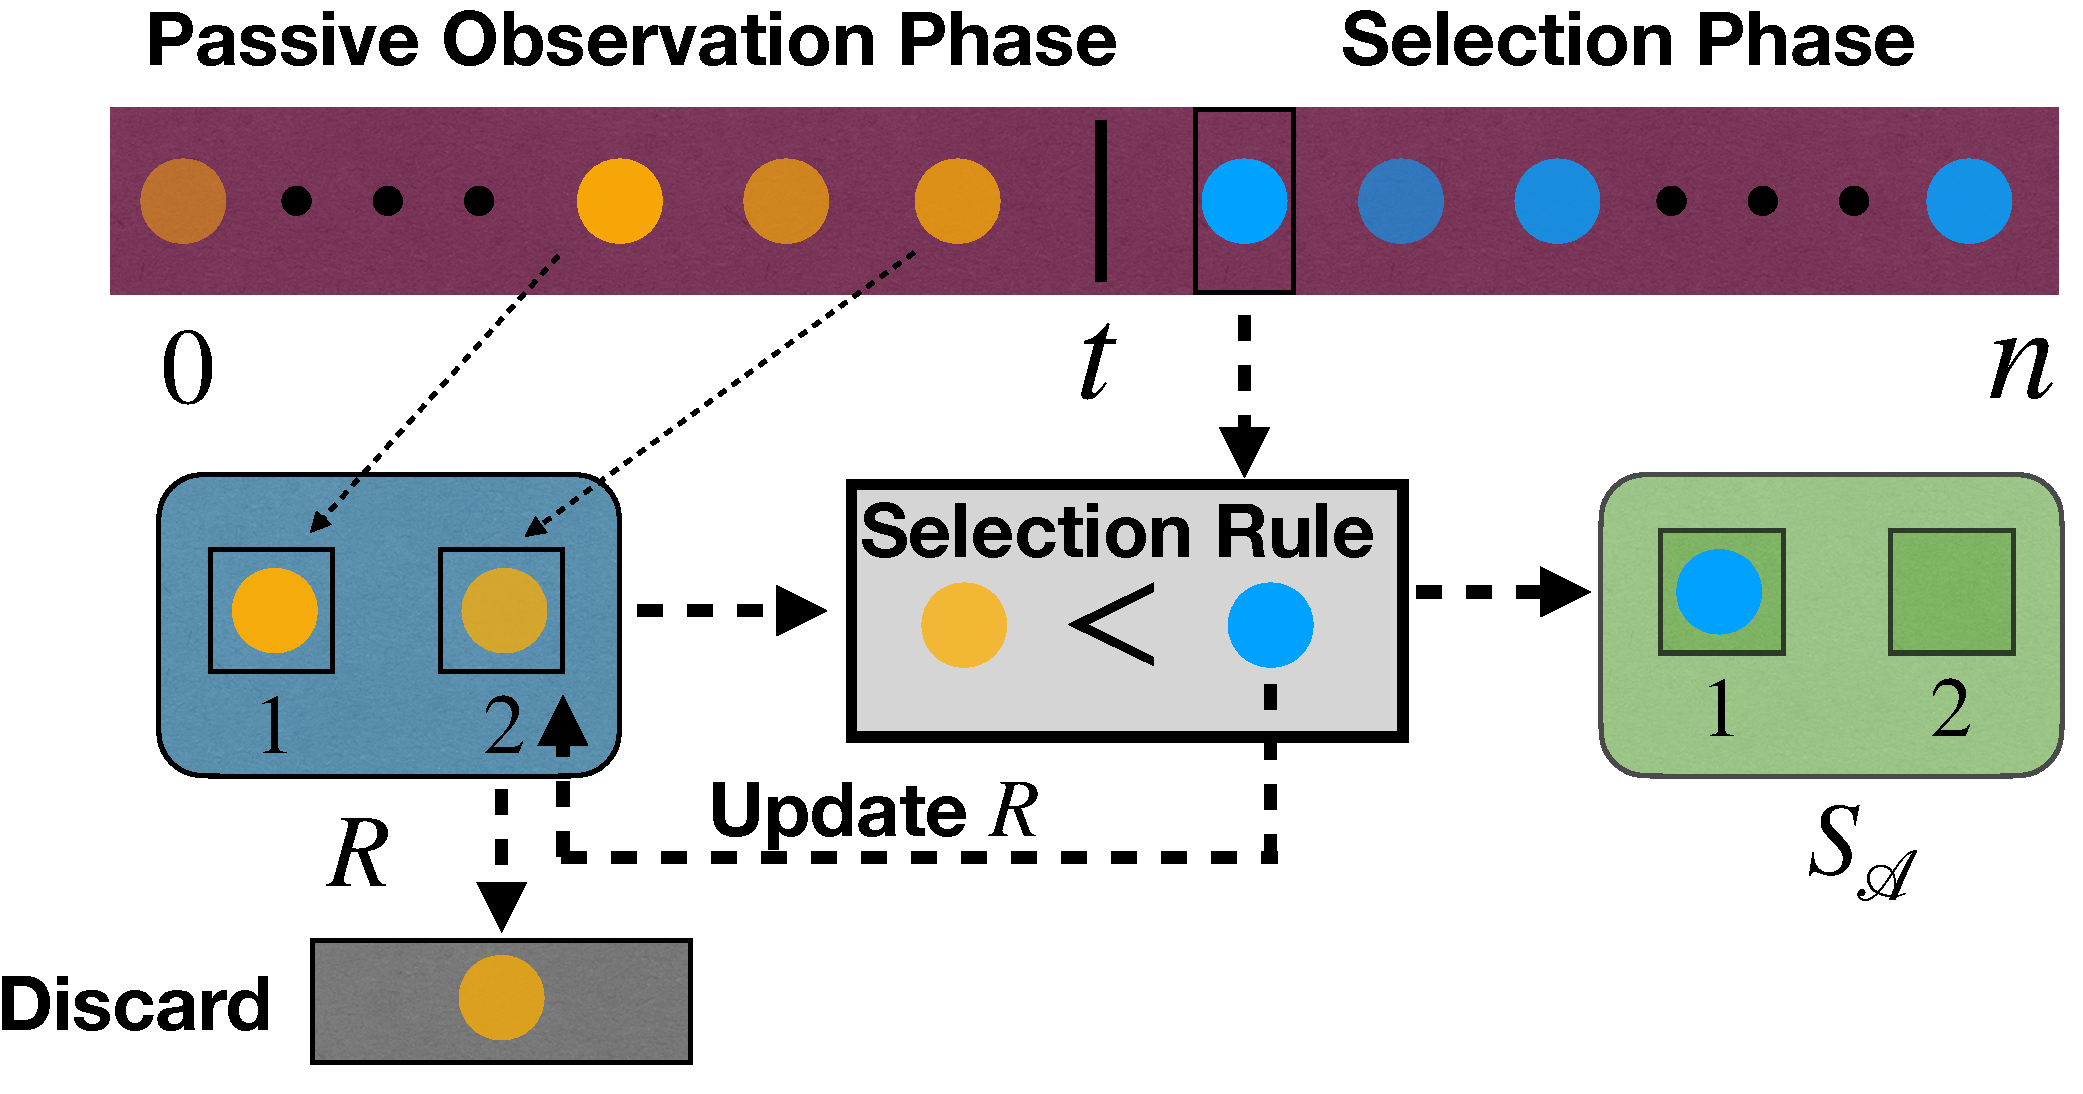
\includegraphics[width=1.01\linewidth]{Figures/Virtual+_algo.pdf}
    \vspace{-10pt}
    \caption{\algoname \ observes $v_i$ (or estimates) and maintains $R$ during the sampling phase. Items are then picked into $S_{\mathcal{A}}$, after threshold $t$, \cut{via comparisons to $R$.}}
    \label{fig:stochastic_secretary}
\end{figure}
\end{minipage}
\cut{
\begin{minipage}[t]{.48\textwidth}
\vspace{0pt}  
    \begin{algorithm}[H]
    \small
    \textbf{Inputs:} Permuted Datastream: $\mathcal{D}_\pi$, Online Algorithm: $\mathcal{A}$,  Surrogate classifier: $f_s$, Target classifier: $f_t$,  Attack method: \textsc{Att}, Loss: $\ell$,  Budget: $k$,  
    Fool rate: $F^{\mathcal{A}}_\pi=0$.
    \begin{algorithmic}[1]
    \FOR{$(x_i,y_i)$ in $\mathcal{D}_\pi$}
    \STATE $x_i' \leftarrow  \textsc{Att}(x_i)$ \hfill \COMMENT{// Compute the attack}
    \STATE $\mathcal{V}_i \leftarrow \ell(f_s(x_i'),y_i)$  \hfill \COMMENT{// Compute the estimate of $v_i$}
    \IF{$\mathcal{A}(\mathcal{V}_1,\ldots, \mathcal{V}_i,k) == \textsc{True}$}
    \STATE  $F^{\mathcal{A}}_\pi \leftarrow F^{\mathcal{A}}_\pi+\tfrac{\mathbf{1}\{f_t(x_i')\neq y_i\}}{k}$  \hfill\COMMENT{// Submit  $x_i'$ on $f_t$} 
    \ENDIF
    \ENDFOR
    \STATE \textbf{return:} $F^{\mathcal{A}}_\pi$ \hfill\COMMENT{// Note that $\mathcal{A}$ always submits $k$ attacks} 
    \end{algorithmic}
     \caption{\small Online Adversarial Attack}
     \label{alg:online_adv_attack}
    \end{algorithm}
\end{minipage}
}


Well known single threshold-based algorithms that solve the $k$-secretary problem include the \textsc{Virtual}, \textsc{Optimistic} \cite{babaioff2007knapsack} and the recent \textsc{Single-Ref} algorithm \cite{albers2020new}. In a nutshell, these online algorithm consists of two phases---a \textit{sampling phase} followed by a \textit{selection phase}---and an optimal stopping point $t$ (threshold) that is used by the algorithm to transition between the phases. In the sampling phase, the algorithms passively observe all data points up to a pre-specified threshold $t$. Note that $t$ itself is algorithm-specific and can be chosen by solving a separate optimization problem. Additionally, each algorithm also maintains a sorted reference list $R$ containing the top-$k$ elements. Each algorithm then executes the selection phase through comparisons of incoming items to those in $R$ and possibly updating $R$ itself in the process (see~\S\ref{appendix:classical_online_algorithms}).

Indeed, the simple structure of both the \textsc{Virtual} and \textsc{Optimistic} algorithms---e.g., having few hyperparameters and not requiring the algorithm to involve Linear Program's for varying values of $n$ and $k$---in addition to being $(1/e)$-competitive (optimal for $k=1$) make them suitable candidates for solving \eqref{eq:asp}. However, 
the competitive ratio of both algorithms in the small $k$ regime---but not $k=1$---has shown to be sub-optimal with \textsc{Single-Ref} provably yielding larger competitive ratios at the cost of an additional hyperparameter selected via combinatorial optimization when $n \to \infty$. 

We now present a novel online algorithm, \algoname, that retains the simple structure of \textsc{Virtual} and \textsc{Optimistic}, with no extra hyperparameters, but leads to a new state-of-the-art competitive ratio for $k<5$. Our key insight is derived from re-examining the selection condition in the \textsc{Virtual} algorithm and noticing that it is overly conservative and can be simplified. The \algoname\ algorithm is presented in Algorithm 1, where the removed condition in \textsc{Virtual} (L2-3) is \st{in pink strikethrough}. Concretely, the condition that is used by \textsc{Virtual} but \emph{not} by \algoname\ updates $R$ during the selection phase without actually picking the item as part of $S_{\mathcal{A}}$. Essentially, this condition is theoretically convenient and leads to a simpler analysis by ensuring that the \textsc{Virtual} algorithm never exceeds $k$ selections in $S_{\mathcal{A}}$. \algoname\ removes this conservative $R$ update criteria in favor of a simple to implement condition, $|S_{\mathcal{A}}| \leq k$ line 4 {\color{salmon}(in pink)}. Furthermore, the new selection rule also retains the simplicity of \textsc{Virtual} leading to a painless application to online attack problems.

\cut{By design, \algoname\ also does not exceed $k$ selections and works for any combination of $k$ and $n$.}
\xhdr{Competitive ratio of \algoname}
What appears to be a minor modification in \textsc{Virtual+} compared to \textsc{Virtual} leads to a significantly more involved analysis but a larger competitive ratio. In Theorem 1, we derive the analytic expression that is a tight lower bound for the competitive ratio of \algoname\ for \emph{general}-$k$. We see that \algoname\ provably improves in competitive ratio for $k<5$ over both \textsc{Virtual}, \textsc{Optimistic}, and in particular the previous best single threshold algorithm, \textsc{Single-Ref}.

\begin{theorem}
The competitive ratio of \algoname\ for $k \geq 2$ with threshold $t_k = \alpha n$ can asymptotically be lower bounded by 
\begin{equation}
    C_k \geq  \max_{\alpha \in [0,1]}  {\alpha}^k \sum_{m = 0}^{k - 1} a_m \ln^m (\alpha)- \alpha a_0
    \quad where  \quad
    a_m := \big(\tfrac{k^k}{(k-1)^{k-m}} - k^m\big)\frac{(-1)^{m+1}}{m!}
    \, .
\end{equation}
Particularly, we get $C_2\geq0.427, C_3\geq .457, C_4\geq.4769$ outperforming~\citet{albers2020new}.
\label{thm:general_k_theorem1}
\end{theorem}

% \begin{proof}[Proof sketch]
% The full proof can be found in \S\ref{appendix:virtual_plus_proof_k_2}. First note that by~\citep[Lem.~3.3]{albers2020new}, we have a competitive ratio for the $k$-secretary problem under any threshold-based algorithm that is equal to 
% \begin{equation}
%   C_n = \tfrac{1}{k}(\mathbb{P}(i_1 \in S_{\mathcal{A}}) + \ldots + \mathbb{P}(i_k \in S_{\mathcal{A}})) \label{eq:C_as_sum_prob}
% \end{equation}
% where $i_a$ is the index of the $a^{th}$ best secretary. 
% Now, let us focus on the case $k=2$.
% When calculating the probability of one of the top-$2$ elements being picked by the algorithm, we must calculate the probability of one of the top-2 elements being picked after the threshold ---i.e., for a given time step $j+1$ between $t+1 \dots n$. A top-$2$ element is picked by \algoname\ if and only if this element appears at that time step and if we haven't already picked $2$ secretaries ($|S_{\mathcal{A}}| < 2$) during the first $j$ steps. Thus, for $a \in \{1,2\}$,
% \begin{align}
%     \mathbb{P}(i_a \in S_{\mathcal{A}}) 
%     % &= \sum_{j=t+1}^n \mathbb{P}(i_a \in S_{\mathcal{A}} \ \text{at time-step }j)  \\
%     &= \tfrac{1}{n}\left(\mathbb{P}_t(|S_{\mathcal{A}}| < 2) +\ldots+ \mathbb{P}_{n-1}(|S_{\mathcal{A}}| < 2)\right)\label{p_picked_equal_not_filled} \notag
% \end{align}
% where $\mathbb{P}_j(E):= \mathbb{P}(E \ \text{in first } j \text{ steps})$ for any event $E$.
% Now, for a given $j$, we compute $\mathbb{P}_j(|S_{\mathcal{A}}| < 2)$ by decomposing the event into the probability of having an empty $S_{\mathcal{A}}$ plus the probability of having $|S_{\mathcal{A}}| = 1$. The computation of the latter is detailed in \S\ref{appendix:virtual_plus_proof_k_2} and summarized in Fig.~\ref{fig:k_2}.
% %\vspace{-1mm}
% \begin{align}
%     \mathbb{P}_j(|S_{\mathcal{A}}| \!=\! 0)
%     =  \tfrac{t(t - 1)}{j (j - 1)},\,
%     \mathbb{P}_j(|S_{\mathcal{A}}| \!=\! 1)
%     = \tfrac{2t}{j(j-1)} \sum_{p = t + 1}^{j}\tfrac{t-1}{p-2} \notag
% %\vspace{-1mm}
% \end{align}
% Overall, by combining the previous equations we get:
% %\vspace{-1mm}
% \begin{equation}
%     C_n = \frac{1}{n}\sum_{j=t}^{n-1}\Big( \frac{t(t - 1)}{j (j - 1)} + 2 \sum_{p = t + 1}^{j}\frac{1}{j}\frac{t}{j - 1}\frac{t-1}{p-2}\Big)
% %\vspace{-1mm}
% \end{equation}
% % \begin{figure}[t]
% %     \centering
% %     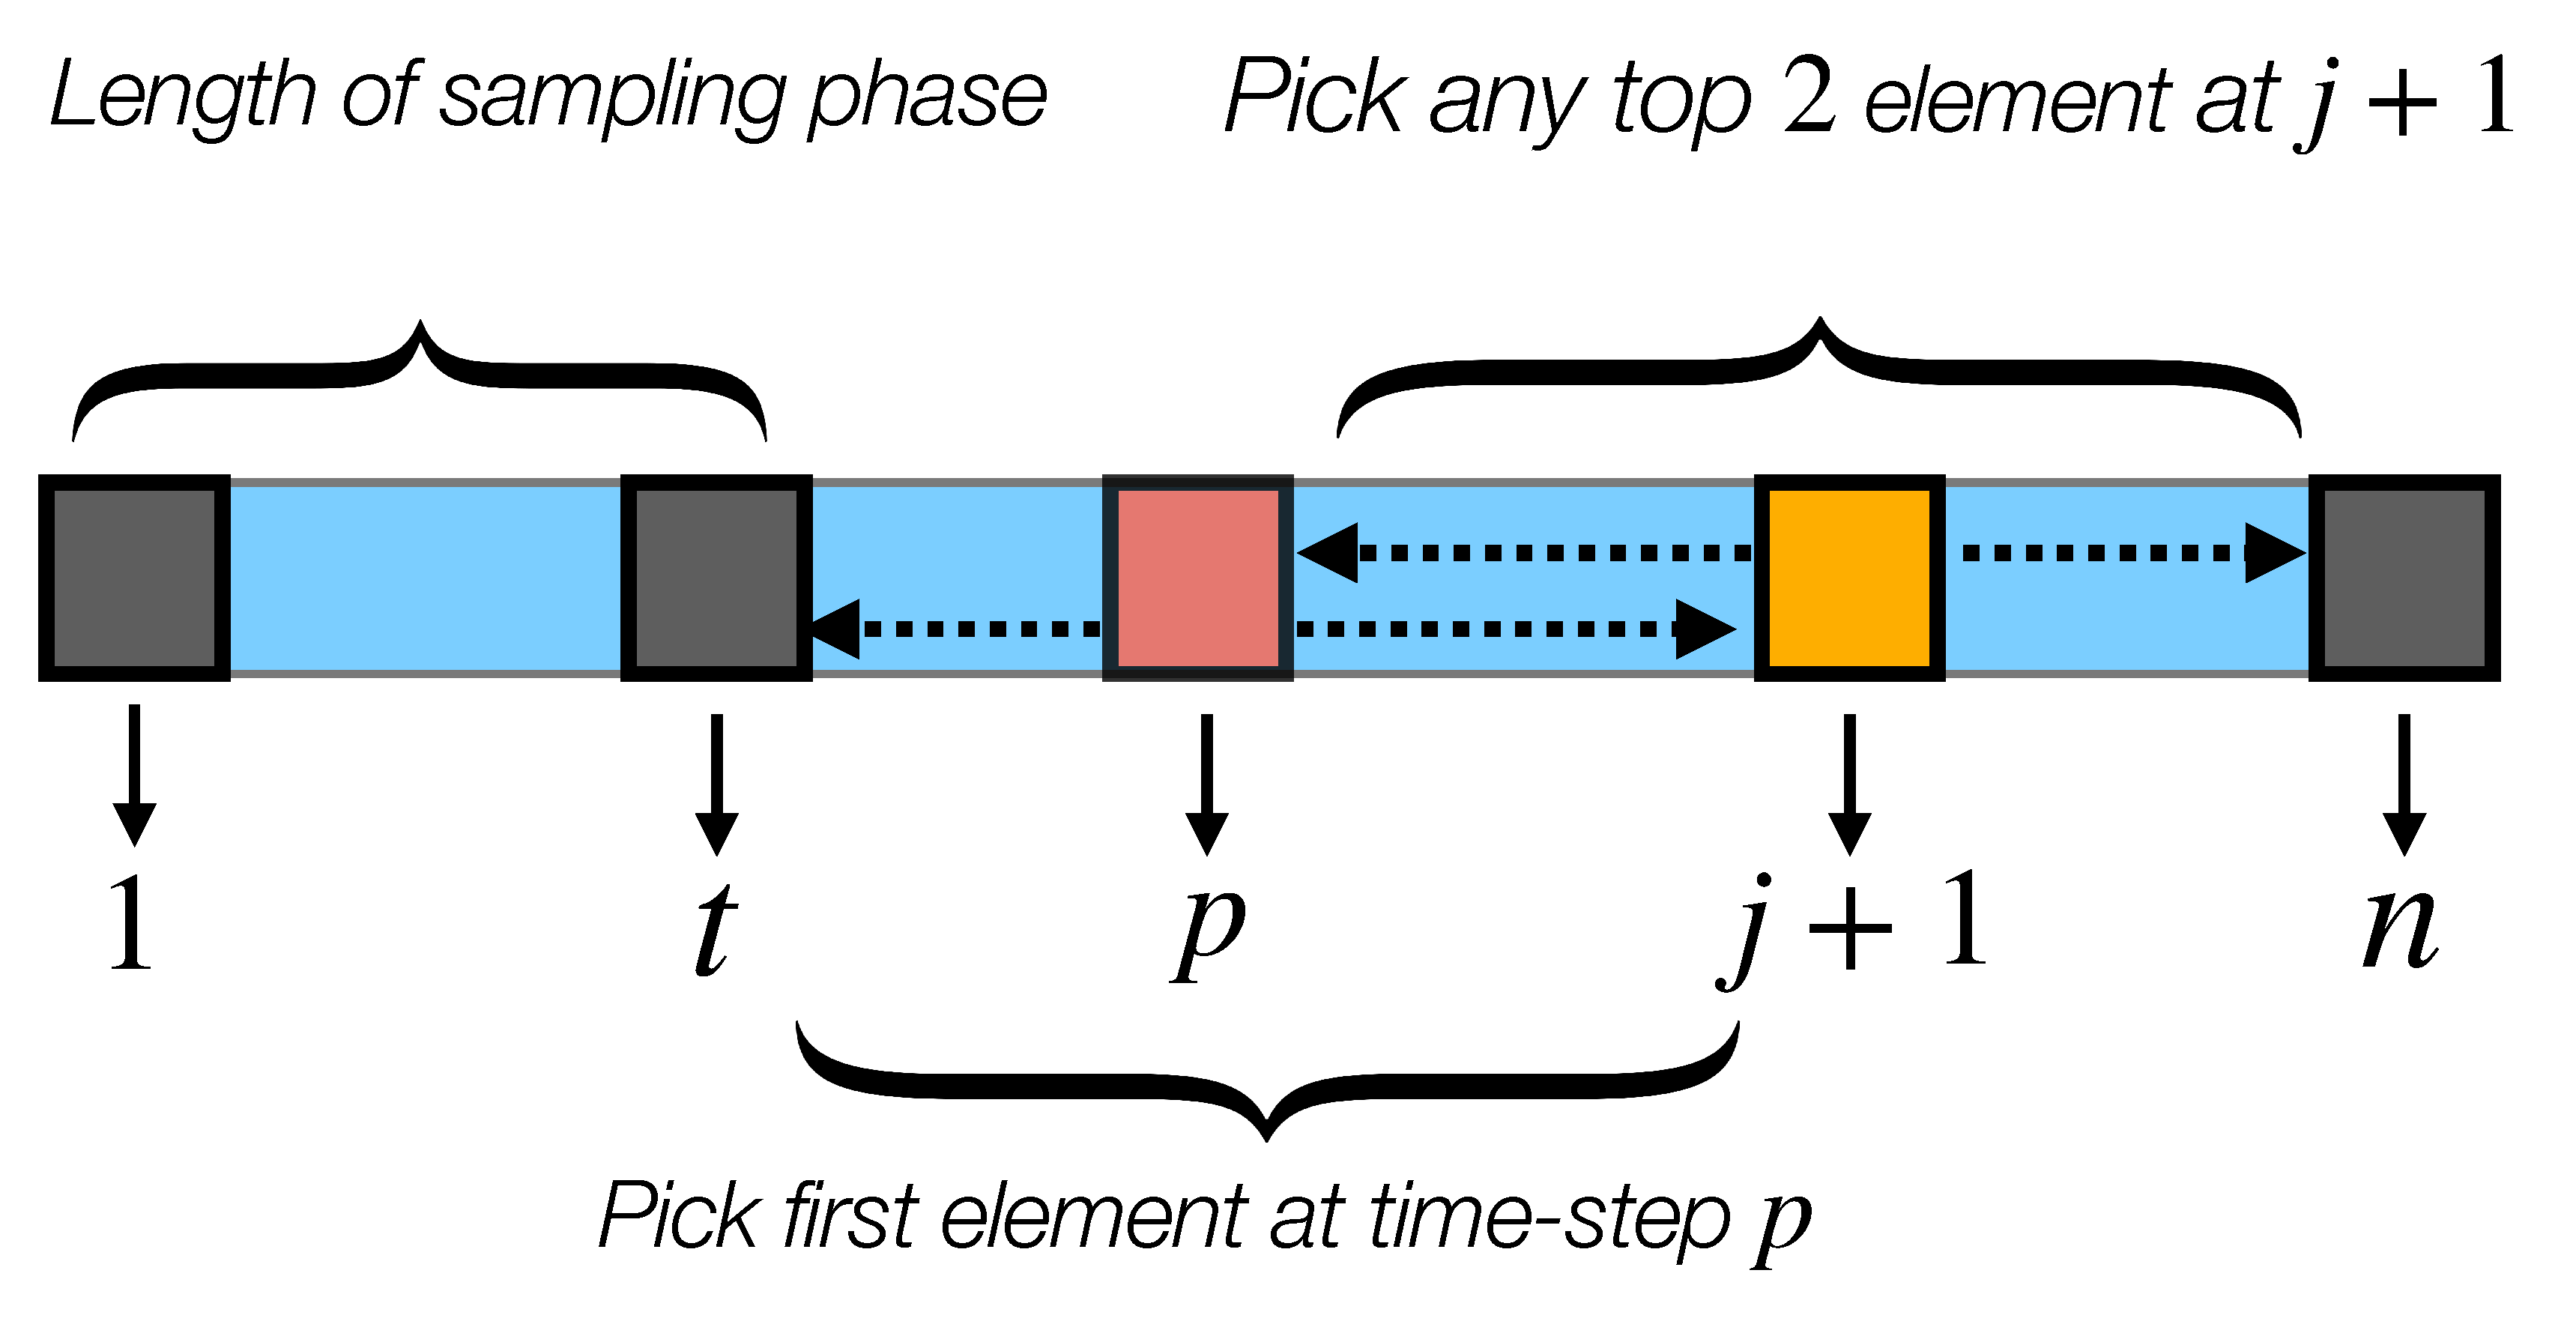
\includegraphics[width=.95\linewidth]{Figures/virtual_plus_k_2.pdf}
% %     \vspace{-15pt}
% %     \caption{Probability of having only one element in $S_{\mathcal{A}}$ after $j$ time-steps with the \algoname algorithm.}
% %     \label{fig:k_2_main}
% %     \vspace{-10pt}
% % \end{figure}
% Finally, by lower bounding the sums with integrals we get, 
% \begin{align}
%     C_n \geq 
%     \tfrac{t(t -1)}{n} \left(\tfrac{3}{t}-\tfrac{2\ln(n/t) + 3}{n} - 2(n-t) \left| \tfrac{16}{3 t^3 e^4} \right|\right) \notag
% %\vspace{-1mm}
% \end{align}
% Now, for $t = \alpha n$ with $\alpha \in (0, 1)$, that lower-bound becomes
% %\vspace{-3mm}
% \begin{equation}
% \label{eq:alpha_eqn}
% C \geq \alpha (3 - \alpha(3 - 2\ln (\alpha))) + \mathcal{O}(1/n) \,,\quad \forall \alpha \in (0,1)
% \end{equation}
% The constant term of the RHS is a concave function of $\alpha$ that is maximized for $\alpha^* \approx 0.38240$. Thus, our algorithms achieves a competitive ratio larger than $0.42737$.
% \end{proof}

\xhdr{Connection to Prior Work}
\label{connection_to_prior_work}
The full proof for Theorem~\ref{thm:general_k_theorem1} can be found in~\S\ref{app:general_k_proof} along with a simple but illustrative proof for $k=2$ in~\S\ref{appendix:virtual_plus_proof_k_2}.
Theorem~\ref{thm:general_k_theorem1} gives a tractable way to compute the competitive ratio of \algoname\ for any $k$, that improve the previous state-of-the-art~\citep{albers2020new} in terms of single threshold $k$-secretary algorithms for $k<5$ and $k>100$.\footnote{\label{foot:closed_form}\citet{albers2020new} only provide competitive ratios of \textsc{Single-Ref} for $k \leq 100$ and conclude that ``a closed formula for the competitive ratio for any value
of $k$ is one direction of future work''. We partially answer this open question by expressing \algoname's optimal threshold $t_k$ as the solution of a uni-dimensional optimization problem. In Table~\ref{tab:C_k}, we provide this threshold for a wide range of $k \geq 100$.} 
However, it is also important to contextualize \algoname\ against recent theoretical advances in this space. 
Most prominently, \citet{buchbinder2014secretary} and \citet{chan2014revealing} proved that the $k$-secretary problem can be solved {\em optimally} (in terms of competitive ratio) using linear programs (LPs), {\em assuming a fixed length of $n$}. But these optimal algorithms are typically not feasible in practice.
Critically, they require individually tuning multiple thresholds by solving a separate LP with $\Omega(n k^2)$ parameters for each length of the data stream $n$, and the number of constraints grows to infinity as  $n\rightarrow\infty$. 
In this work, we focus on practical methods with a \emph{single} threshold (e.g. Algorithm~\ref{alg:virtual_plus}) that do not require involved computations that grow with $n$. 



